% !TeX root = main.tex
\lecture{3}{Thu 29 Jan 2026 15:00}{Mechanics III: Moment of Inertia}

\section{Moments of Inertia Examples}
\subsection{Point Mass on a Light Ring}
Consider a point mass on a light ring. The ring has radius $R$ and the point masses axis of rotation runs through the ring centre. 

This is trivially:
\[
    I = mR^2
\]

\subsection{Uniform Ring}
Consider the same example, but instead of a point mass the ring is massive, with mass $M$. All of the mass still sits at the same distance from the axis of rotation.

Hence it is still $I = MR^2s$.

\section{Uniform Solid Disk}
Consider a uniform solid disk of radius $R$ and constant mass density $\rho$. Similar to CoM problems we need to break it down and consider the object as being a sum over multiple elements, $i$.

\[
    I = \sum_i m_i r_i^2
\]

As the size of each element becomes infinitesimal, this becomes an integral:
\[
    I = \int dI = \int r^2 dm
\]
To make this integral easier we want to think of elements at a fixed $r$, i.e. considering infinitesimal rings.

\section{Thick Solid Disk}
Consider a disk now being $3D$, with height $h$. The mass element for each infinitesimal ring is now:
\[
    dm = \rho dV = \rho h \left(\pi (r + dr)^2 - \pi r^2\right)
\]

Expanding and disregarding the $dr^2$ term:
\[
= \rho h 2 \pi r dr
\]

Hence for the ring, the contribution to the moment of inertia is:
\[
    dI = r^2 dm = 2 \pi \rho h r^3 dr
\]

And integrating:
\[
    I = \int_{0}^{R} \, dI = \int_{0}^{R} 2 \pi \rho h r^3 \, dr
\]
\[
    = 2 \pi \rho h \left[r^4 / 4\right]_0^R = \frac{\pi \rho h R^3}{2}
\]

And to swap from density into mass we use $M = \rho V$:
\[
    \rho = \frac{M}{V} = \frac{M}{\pi R^2 h}
\]

Hence:
\[
    \boxed{I = \frac{\pi h R^4}{2} \times \frac{M}{\pi R^2 h} = \frac{MR^2}{2}}
\]

\section{Parallel Axis Theorem}
So far, we assume that the axis of rotation is collinear with the centre of mass. However, we may care about the moment of inertia passing through an axis which does not pass through the CoM (or indeed the object itself). Rather than doing it manually, we can make a shortcut if we know the result for the moment of inertia through a parallel axis through the CoM.

Consider an arbitrary shaped object with axis $A_0$ through the CoM, $I_0$. Consider a parallel axis $A$ outside of the object, $I$. 

The distance between the axis is given as $R$. We select a coordinate system with the origin at the CoM.

\begin{figure}[H]
    \centering
    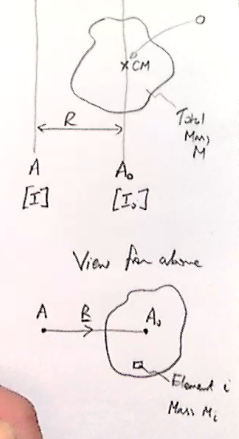
\includegraphics[width=0.25\textwidth]{figures/lec03_01.png}
     \caption{}
\end{figure}

Define $r_i$ as the vector between $A$ (at the same vertical position) and a random point in the object, and $r_i^0$ being the vector from $A_0$ to the same point.

\[
    I_A = \sum_i m_i \vec{r}_i^2
\]

By vector addition:
\[
    I_A = \sum_i m_i \left(\vec{R} + \vec{r}_i^0\right)^2
\]
\[
    = \sum_{i}^{} m_i \left(R^2 + {r_i^0}^2 + 2 \vec{R} \cdot \vec{r}_i^0\right)
\]

$R$ is constant, hence:
\[
    I_A = R^2 \sum_i m_i + \sum_i m_i {r_i^0}^2 + 2R \cdot \sum m_i
\]
\[
    = R^2 M + I_0 + 2 \vec{R} \cdot \sum m_i \left(\vec{r}_i^{\,0}\right)^2
\]

However we define the centre of mass with (noting we defined the origin at the CoM):
\[
    r_\text{CM} = 0 = \frac{\sigma_i m_i r_i^0}{M}
\]

So:
\[
    \sigma_i m_i \left(\vec{r}_i^{\,0}\right)^2 = 0
\]

Hence finally:
\[
    I_A = I_0 + MR^2
\]

